\section{Verwendete Werkzeuge}
\subsection{Bugtracker}
Um die Kommunikation innerhalb des Teams zu erleichtern und stets problembezogen zu gestalten wurde bereits während der Implementierungsphase  die Bugtracking-Software ``github Issues'' eingesetzt. Diese ist mit dem Quellcode-Repository integriert, sodass aus dem Bugtracker einfach auf Änderungen im Code verwiesen werden kann und sogar durch einen Eintrag in der Mitteilung zu einem Commit eine solche Referenz automatisch erzeugt werden kann.

Über den gesamten Entwicklungszeitraum hinweg wurden knapp über 100 Bugs angelegt. Davon bezogen sich etwa 30 auf die Benutzeroberfläche und jeweils ca. 20 auf die Beweiserschnittstelle und den Interpreter.

\subsection{Continous-Integration Server}
Die Continous-Integration Serversoftware Jenkins, die bereits während der Implementierungsphase verwendet wurde, um nach jeder Änderung die Kompilierbarkeit des Codes zu überprüfen, wurde auch in der Validierungsphase eingesetzt. Dabei wurden zusätzlich Plugins verwendet, die die Anzahl der Testfälle sowie die Anzahl der momentan erfolgreichen Tests grafisch anzeigen.

\begin{center}
	\begin{figure}[h] % place the figure here
		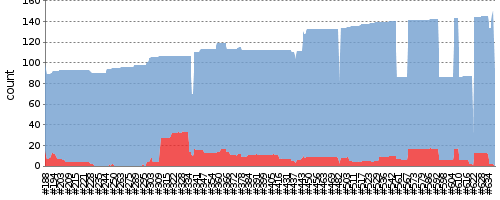
\includegraphics[width=13cm]{images/jenkins-test-trend.png}
		\caption{Entwicklung der Anzahl von Testfällen während der Validierungsphase}
	\end{figure}
\end{center}
